%*******************************************************************************
%*******************************************************************************
\chapter{Songbook-Client}
\setcounter{chapter}{2}
\label{chap:songbook-client}
\minitoc
\newpage
%*******************************************************************************
%*******************************************************************************

Le Songbook-Client est interface graphique facilitant la création de
recueils de chansons
personnalisés\footnote{\url{http://www.ohloh.net/p/songbook-client},
  \url{http://github.com/crep4ever/songbook-client}}.

\begin{nota}
Quelle que soit votre plateforme, il est nécessaire d'avoir installé
au préalable les dépendances du songbook lui-même
(\refsec{sec:install}) afin de pouvoir produire un recueil \ext{pdf}.
\end{nota}

Les téléchargements suivant les différents systèmes d'exploitation
sont proposés sur \url{http://www.patacrep.com/static1/downloads}.


%*******************************************************************************
\section{Interface}
%*******************************************************************************

%-------------------------------------------------------------------------------
\subsection{Premier lancement}
%-------------------------------------------------------------------------------

\begin{figure}
  \centering
  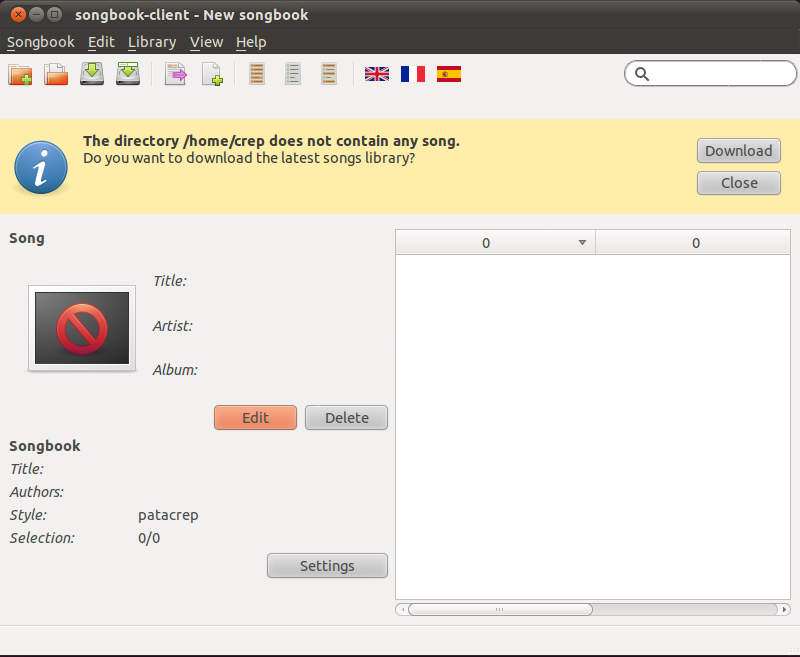
\includegraphics[width=.7\textwidth]{start}
  \caption{Premier lancement de l'application \client.}
  \label{fig:start}
\end{figure}

Par défaut, l'interface est vide (\reffig{fig:start}). Le
songbook-client doit être lié à un \emph{songbook} existant. Vous avez
deux solutions~:

\begin{enumerate}
\item indiquer le chemin d'un répertoire \directory{songbook} existant
  depuis le menu \menu{Édition}{Préférences}
  (\reffig{fig:solution-a})~;
\item télécharger la dernière version depuis internet depuis le menu
  \menu{Bibliothèque}{Télécharger} (\reffig{fig:solution-b}).
\end{enumerate}

%%%%%%%%%%%%%%%%%%%%%%%%%%%%%% FIGURE %%%%%%%%%%%%%%%%%%%%%%%%%%%%%%%%%%
\begin{figure}
  \centering
  %% -- subfigures --
  \subfigure[]{
    \label{fig:solution-a}
    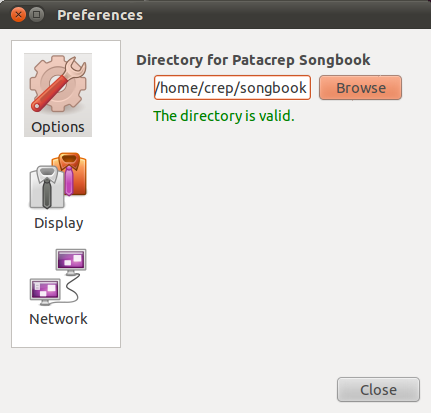
\includegraphics[width=0.45\textwidth]{preferences}%
  }%
  \hspace{0.1cm}%
  \subfigure[]{%
    \label{fig:solution-b}%
    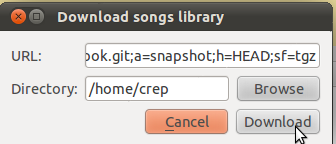
\includegraphics[width=0.45\textwidth]{download}%
  }%
  %% -- subfigures --
  \caption[Lier]{% 
    Deux solutions permettent de lier l'application à un \emph{songbook}.
    \subref{fig:solution-a}~Indiquer le chemin d'un répertoire existant~;%
    \subref{fig:solution-b}~Télécharger depuis internet.%
  }%
  \label{fig:solutions}
\end{figure}
%%%%%%%%%%%%%%%%%%%%%%%%%%%%%%%%%%%%%%%%%%%%%%%%%%%%%%%%%%%%%%%%%%%%%%%%

Après avoir indiqué ou téléchargé un \recueil, le \client génère la
\emph{bibliothèque des chansons} trouvées dans le sous-répertoire
\directory{songs} du \recueil.

%-------------------------------------------------------------------------------
\subsection{La bibliothèque des chansons}
%-------------------------------------------------------------------------------

\begin{figure}
  \centering
  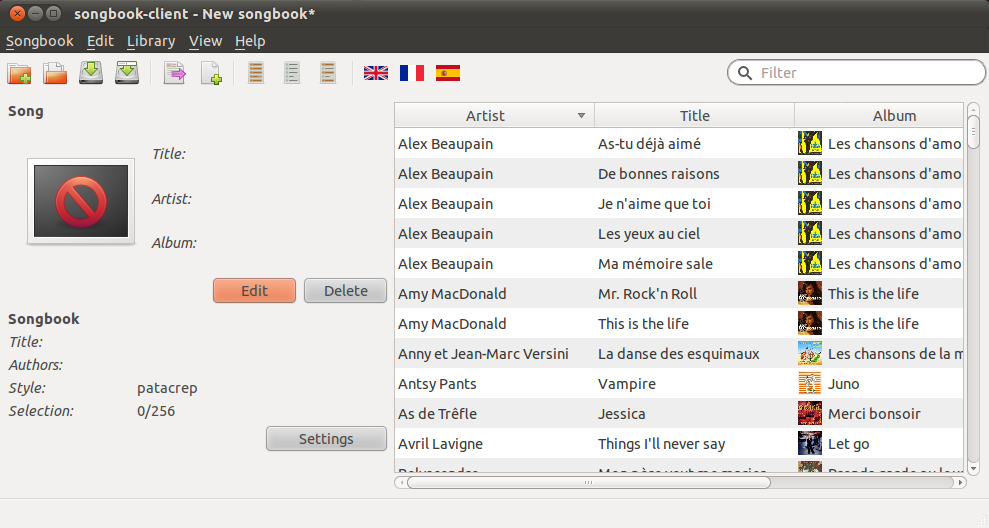
\includegraphics[width=.7\textwidth]{library}
  \caption{La bibliothèque des chansons.}
  \label{fig:library}
\end{figure}

L'ensemble des chansons \ext{sg} trouvées dans le sous-répertoire
\directory{songs} est présenté sous la forme d'une liste. Les
différentes colonnes peuvent être affichées/masquées dans l'onglet
\menu{Affichage} du menu \menu{Édition}{Préférences}. Par défaut,
seules les colonnes \command{Titre}, \command{Artiste} et
\command{Album} sont visibles.

Les chansons de la bibliothèque sont sélectionnables par simple clic.
Une chanson sélectionnée est affichée en surbrillance. Cliquez sur une
chanson sélectionnée pour la désélectionner.

%*******************************************************************************
\section{Ajouter une chanson}
%*******************************************************************************

Le menu \menu{Bibliothèque}{Nouvelle chanson} permet d'ajouter une
nouvelle chanson à la bibliothèque (\reffig{fig:new-song-a}). La boîte
de dialogue permet de renseigner les méta-données de la chanson comme
son titre, son compositeur etc. Ces différents champs permettent de
générer le squelette du nouveau fichier \ext{sg} correspondant à la
chanson (\reffig{fig:new-song-b}). La troisième étape
(\reffig{fig:new-song-c}) consiste à écrire la tablature. Enfin, la
chanson peut être sélectionnée dans la bibliothèque pour en obtenir le
rendu au format pdf depuis le menu \menu{Recueil}{Générer PDF}
(\reffig{fig:new-song-d}).

%%%%%%%%%%%%%%%%%%%%%%%%%%%%%% FIGURE %%%%%%%%%%%%%%%%%%%%%%%%%%%%%%%%%%
\begin{figure}
  \centering
  %% -- subfigures --
  \subfigure[]{
    \label{fig:new-song-a}
    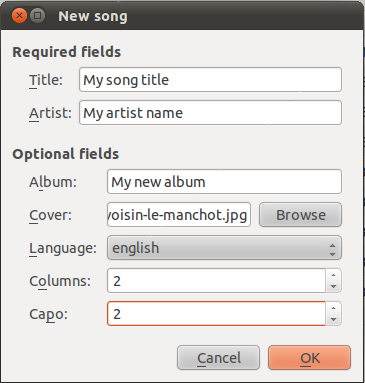
\includegraphics[width=0.35\textwidth]{new-song}%
  }%
  \hspace{0.1cm}%
  \subfigure[]{%
    \label{fig:new-song-b}%
    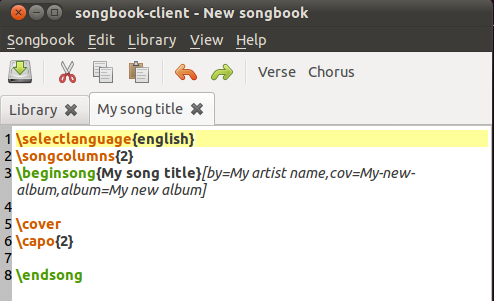
\includegraphics[width=0.6\textwidth]{song-editor-1}%
  }%
  \hspace{0.1cm}%
  \subfigure[]{%
    \label{fig:new-song-c}%
    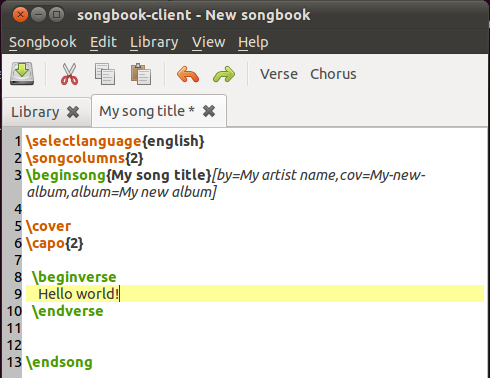
\includegraphics[width=0.6\textwidth]{song-editor-2}%
  }%
  \hspace{0.1cm}%
  \subfigure[]{%
    \label{fig:new-song-d}%
    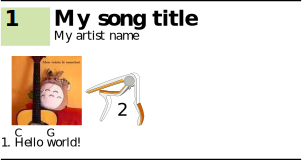
\includegraphics[width=0.35\textwidth]{result}%
  }%
  %% -- subfigures --
  \caption{%
    Ajout d'une nouvelle chanson.
    \subref{fig:new-song-a}~Renseignement des méta-données~; %
    \subref{fig:new-song-b}~Génération automatique du squelette \ext{sg}~; %
    \subref{fig:new-song-c}~Écriture de la tablature~; %
    \subref{fig:new-song-d}~Génération du pdf.%
  }%
  \label{fig:new-song}
\end{figure}
%%%%%%%%%%%%%%%%%%%%%%%%%%%%%%%%%%%%%%%%%%%%%%%%%%%%%%%%%%%%%%%%%%%%%%%%


%*******************************************************************************
\section{Création d'un recueil personnalisé}
%*******************************************************************************

\paragraph{Enregistrement/Ouverture}
Le format de fichier \ext{sb} enregistre la liste des chansons
sélectionnées ainsi que son style et ses options
(voir~\refsec{sec:create-songbook}).

\paragraph{Style et options d'un recueil}
Une boîte de dialogue permet de rapidement sélectionner le style du
recueil pdf ainsi que les différentes éléments à afficher
(\reffig{fig:new-songbook}).

\begin{figure}
  \centering
  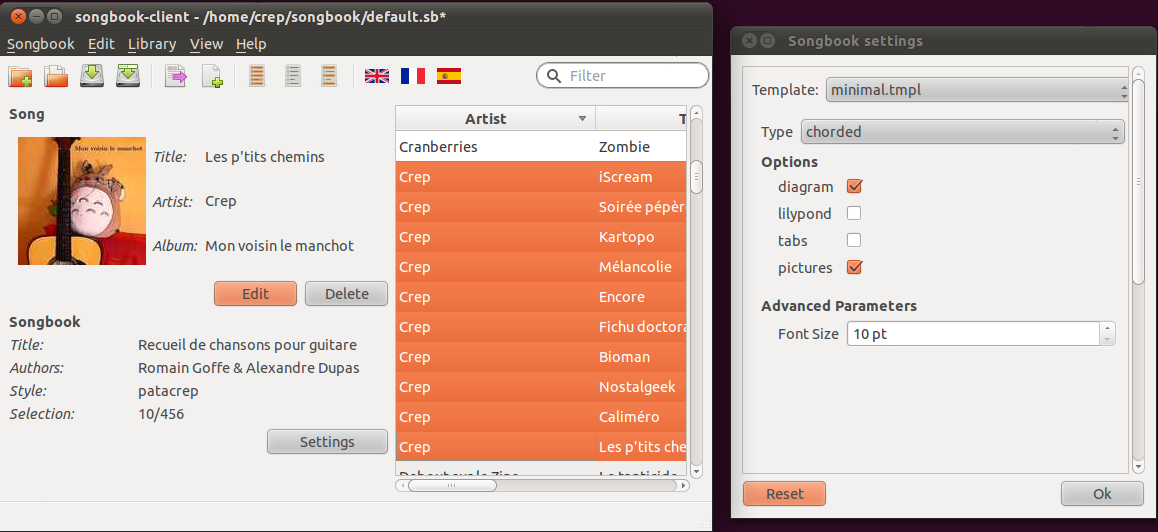
\includegraphics[width=\textwidth]{new-songbook}
  \caption{Personnalisation d'un recueil.}
  \label{fig:new-songbook}
\end{figure}

%*******************************************************************************
\section{Compilation depuis les sources}
%*******************************************************************************

%-------------------------------------------------------------------------------
\subsection{\linux}
%-------------------------------------------------------------------------------

\paragraph{Compilation depuis les sources}

\begin{unix}
  sudo apt-get install build-essential cmake libarchive-dev
  sudo apt-get install qt4-qmake qt4-dev-tools libqt4-sql-sqlite
\end{unix}

\begin{unix}
  git clone git://github.com/crep4ever/songbook-client.git
  cd songbook-client
  make && sudo make install
\end{unix}

%-------------------------------------------------------------------------------
\subsection{\windows}
%-------------------------------------------------------------------------------


%*******************************************************************************
\section{FAQ}
%*******************************************************************************

\paragraph{Comment signaler un bug ?}
Directement sur Github
(\url{http://github.com/crep4ever/songbook-client/issues}) ou via le
forum (\url{http://www.patacrep.com/forum/}).

\paragraph{Erreur Sqlite au démarrage} 
Si vous voyez une boîte de dialogue d'avertissement se lancer au
démarrage de l'application indiquant que le support de sqlite est
nécessaire, vous ne pourrez pas utiliser l'interface. Vérifiez que
votre système dispose bien du support Qt de sqlite (sous
Debian/Ubuntu, il s'agit du paquet \command{libqt4-sql-sqlite}).

\paragraph{Les partitions de solfège n'apparaissent pas}
Si la compilation de votre recueil de chansons n'intègre pas les
partitions malgré l'option \emph{Lilypond} correctement cochée dans les
préférences, vérifiez que Lilypond est bien installé sur votre système. 

\paragraph{La bibliothèque des chansons est vide} 
Vérifiez que le chemin d'accès au patacrep songbook est correctement
renseigné dans Édition/Préférences.  Le chemin indiqué doit contenir
impérativement le makefile et le répertoire \directory{songs/}.

\paragraph{Erreurs après renommage/suppression d'une chanson} 
Un \command{make clean} ou, depuis l'interface, Recueil/Nettoyer devrait
régler le problème. S'il persiste encore, une solution radicale
consiste à supprimer manuellement tous les fichiers \ext{d} présents
dans \directory{$\sim$/songbook}.
